\documentclass[12pt,twoside]{article}

%%%%%%% Loading packages and macros %%%%%%%
\usepackage{preamble/__packages__}
\usepackage{preamble/__macro__}
%%%%%%%%%%%%%%%%%%%%%%%%%%%%%%%%%%%%%%%%%%%

%%%%%%% Document %%%%%%%
\newcommand{\assignment}{Assignment 5}
\newcommand{\course}{FINC 585-3: Asset Pricing}
\newcommand{\prof}{Torben Andersen}
\newcommand{\institute}{Kellogg School of Management}

\title{\course-\assignment}
\author{TA: Jose Antunes-Neto}
\date{\today}
%%%%%%%%%%%%%%%%%%%%%%%%

\begin{document}
\maketitle

The objective of this assignment is for you to gain some familiarity with basic features of the high- frequency return data. You should use the data posted on the canvas site for the S\&P 500 ETF labelled the “spider” or SPY. It provides the index values at a one-minute frequency. Use the sample from February 1993 through January of 2023. The data are available both as \textit{csv} and \textit{mat} formatted files. Downloading this large file as csv may require a large degree of memory. Contact the T.A., Jose, if you have trouble obtaining the full series.

\begin{enumerate}[label = \arabic*)]
    \item Construct the average trading day realized volatility (\textbf{RV}) across all trading days over the Feb 1993 -- Jan 2023 sampel for a variety of underlying sampling frequencies. That is, you should cumulate the daily squared returns from the market open to market close each trading day and then average them across all trading days. This becomes a measure of the average (unconditional) trading-day return variation across the sample. A reasonable choice is to compute measures for the 1-min, 2-min, 3-min, 5-min, 7-min, 10-min, 15-min, 20-min, 25-min, 30-min, 45-min and 60-min frequency. If the frequency does not ``fit'', so there is a small interval left at the end of the trading day, please just add the squared return for this period to the others for the trading day, i.e., if 5 minutes are left over when sampling each 7-min, then the last term is a squared 5-minute return. Plot the values obtained for the average daily trading day RV as a function of the sampling frequency (1-min up to 60-min, say). This becomes a ``vol signature plot';. Does the plot have an approximately ``flat'' region across some frequencies?
    \begin{solution}
        The file \textit{SPY\_HF.csv} contains 1-minute returns from 1993-2023 for the S\&P 500 ETF. I use the log returns to study the volatility of the series. Given a sampling frequency, I cumulate the returns to upsample our series to the desired frequency and then use this series to compute the realized volatility measure. 

        For the sampling frequency, I use a sequence from 1 to 60 minutes with a step of 1 minute. As seen in the lecture notes, the volatility estimator tends to diverge as \(\Delta \to 0\) as the microstructure noise in the data starts to dominate in very high frequencies. This is exemplified in Figure~\ref{fig:volatility_signature}. This figure plots the average daily volatility as a function of the sampling frequency as well as an exponential trend. We can see that the volatility is approximately constant for frequencies between 1 and 20 minutes and it starts to exponentially rise due to the microstructure noise.

        \begin{figure}[!htbp]
            \centering
            \caption{Volatility Signature Plot}
            \label{fig:volatility_signature}
            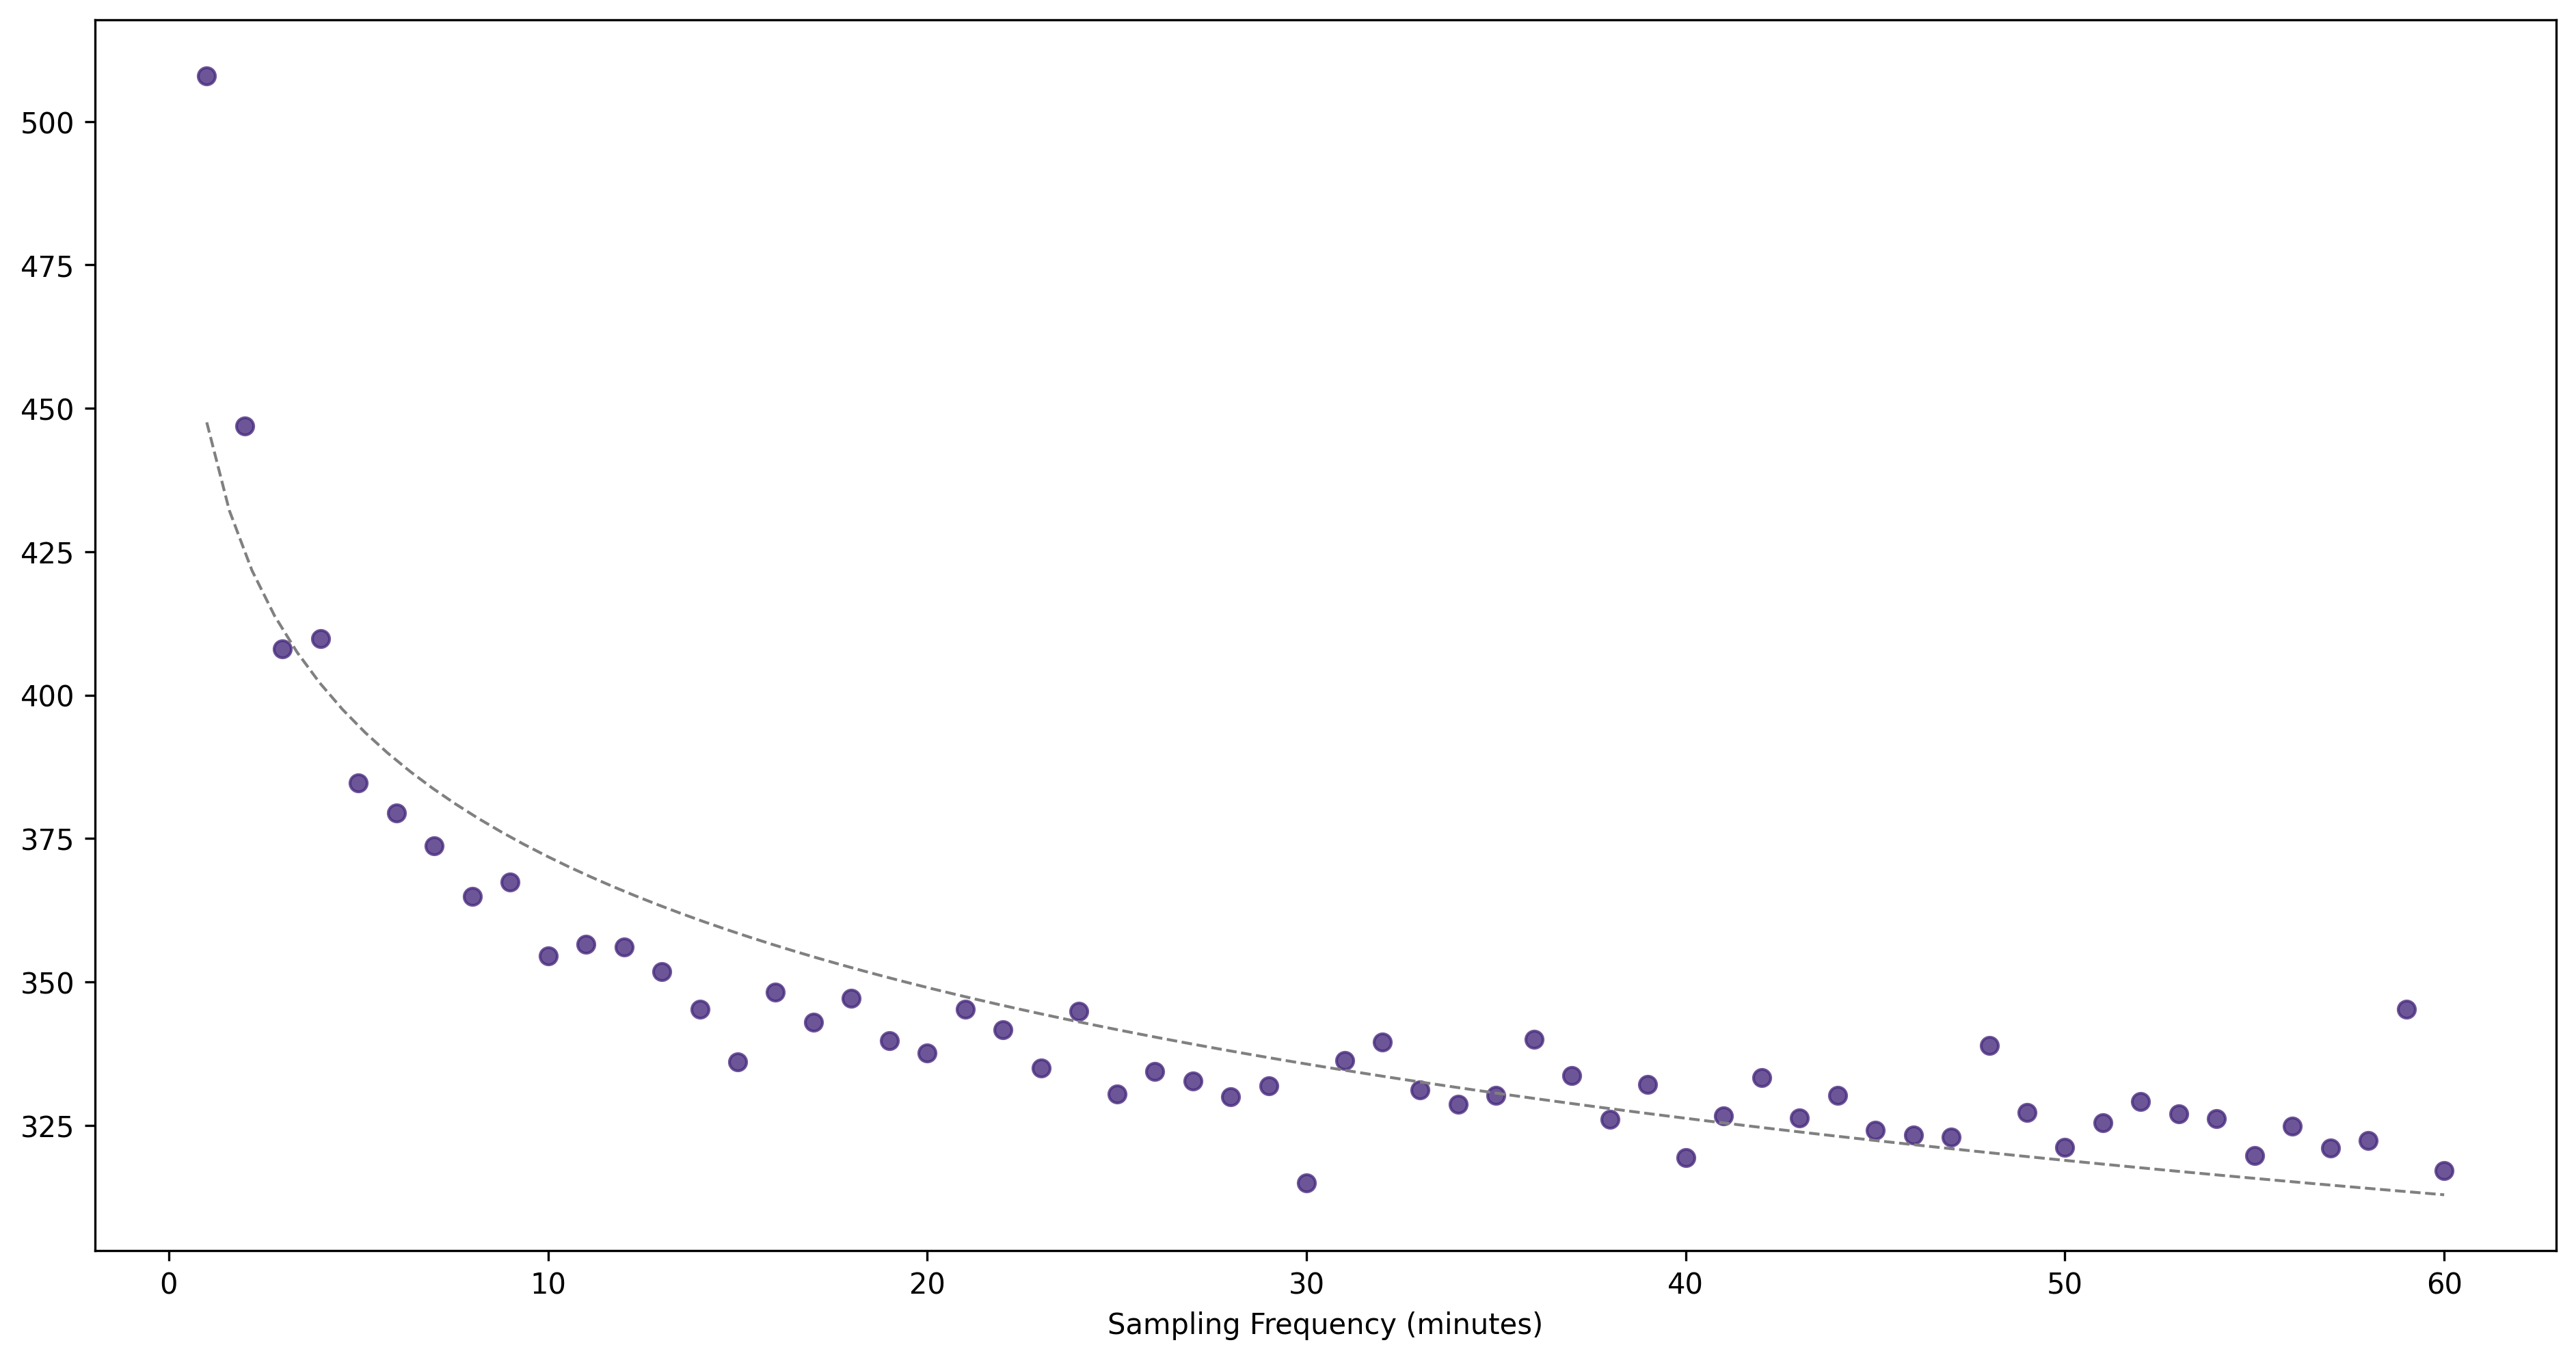
\includegraphics[width=.8\textwidth]{images/volatility_signature.png}
        \end{figure}
        
    \end{solution}
    \item For each one-minute return across the trading day, please compute the average absolute return across all trading days in the sample for this interval, and repeat for all one-minute intervals in the trading day. Plot the value against the time-of-day from the open until the close of the trading day. This figure represents the intraday volatility pattern.
    \begin{solution}
        This question will study the U-shape pattern of volatility. This phenomenom states that the market volatility is higher in the first and last hours of the trading day, and lower in the middle of the day. This is due to the fact that the market is more active in the first and last hours of the day, and less active in the middle of the day. 

        To understand this, I group the observations by the minute of the day and compute the average absolute return for each of these minutes. The NYSE TAQ database follows the Eastern Time Zone. So market hours are from 9:30 to 16:00. The first minutes of the trading day display very high noise due to the high inflow of information in the overnight. For this reason, I exclude the first 30 minutes in my analysis and only consider the information starting at 10am. 
        
        The results are shown in Figure~\ref{fig:volatility_smile}. We can see that the volatility is higher in the first and last hours of the day, and lower in the middle of the day. This is consistent with the volatility smile stylized fact. Moreover, they seem to exhibit some seasonality, with the volatility spiking up at every 30 minutes. 

        \begin{figure}[!htbp]
            \centering
            \caption{Intraday Volatility Pattern}
            \label{fig:volatility_smile}
            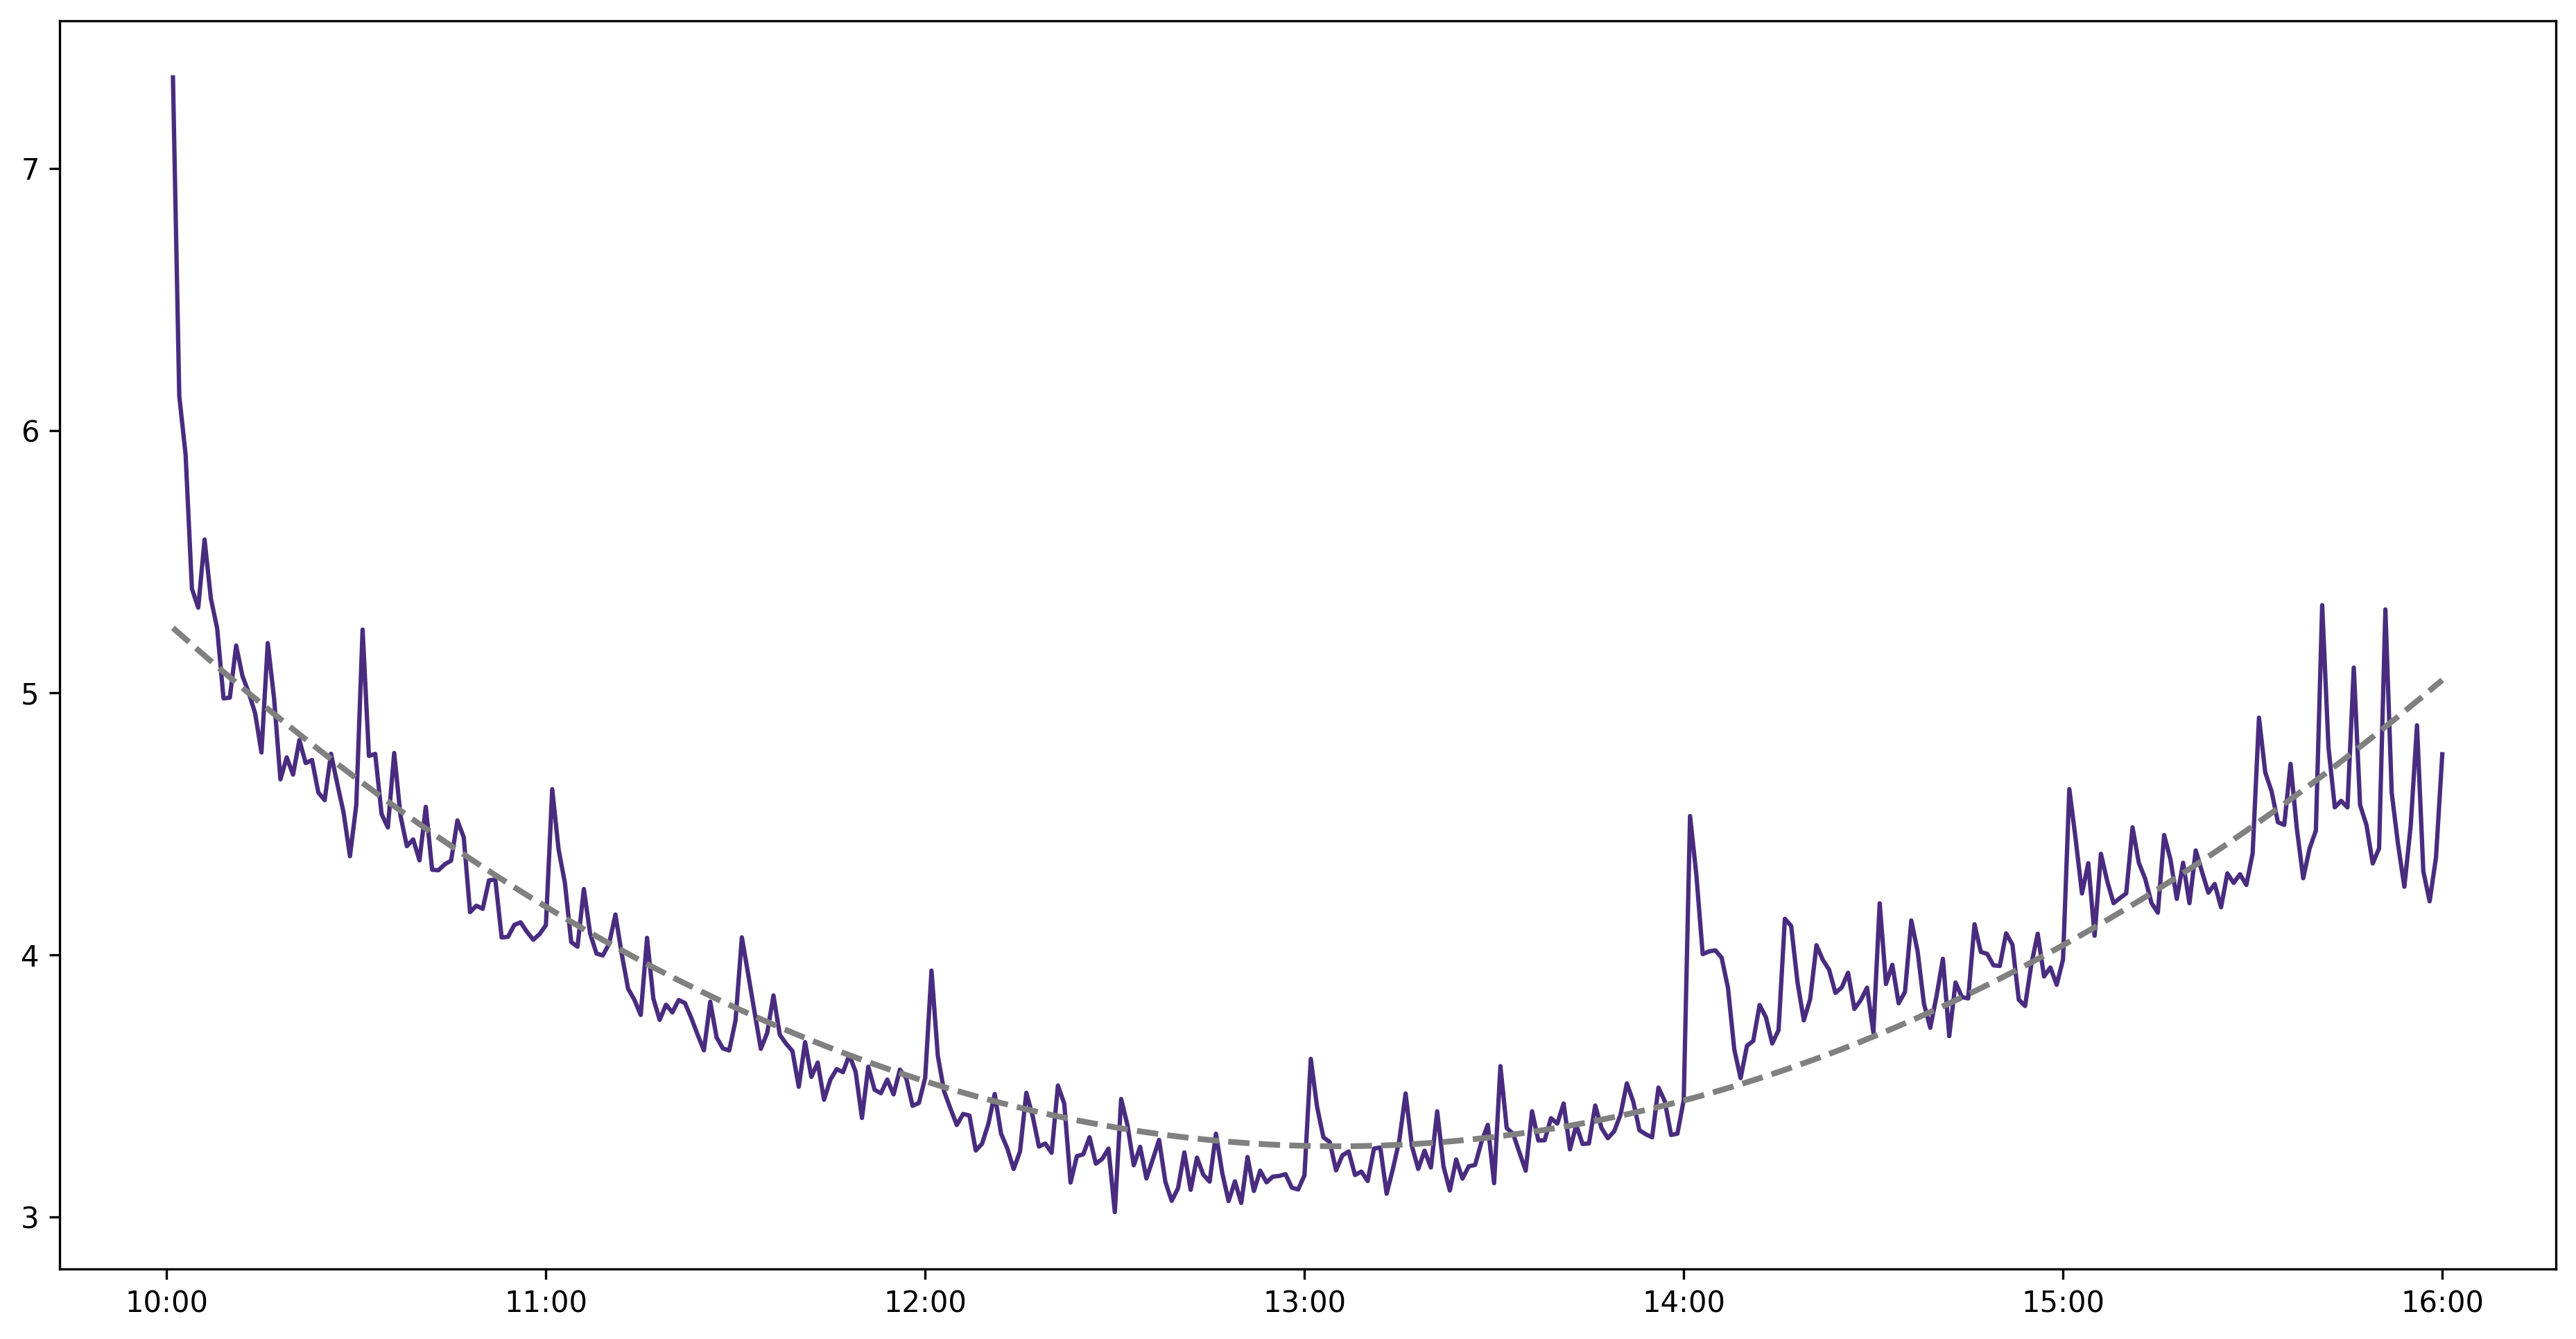
\includegraphics[width=.8\textwidth]{images/intraday_vol.png}
        \end{figure}

    \end{solution}
    \item Compute the measures in question 2) for each of the first two full years of the sample and for the last two full years of the sample. Please plot them as indicated in question 2).
    
    \begin{solution}
        We now turn to analyze how did the volatility smile changed in the last 30 years. Similar to Question 2, I plot the intraday volatility pattern for the years of 1994-1995 and 2021-2022. The results are shown in Figure~\ref{fig:volatility_smile_firstlast}. The intraday volatility for the recent years seems way higher than the volatility in the 90s. However, the intraday pattern is the same for both of them. It is also interesting to note that the intraday volatility for the years of 2021-2022 seems to have a higher value around 2pm.

        \begin{figure}[!htbp]
            \centering
            \caption{Changes in the Intraday Volatility Pattern over the years}
            \label{fig:volatility_smile_firstlast}
            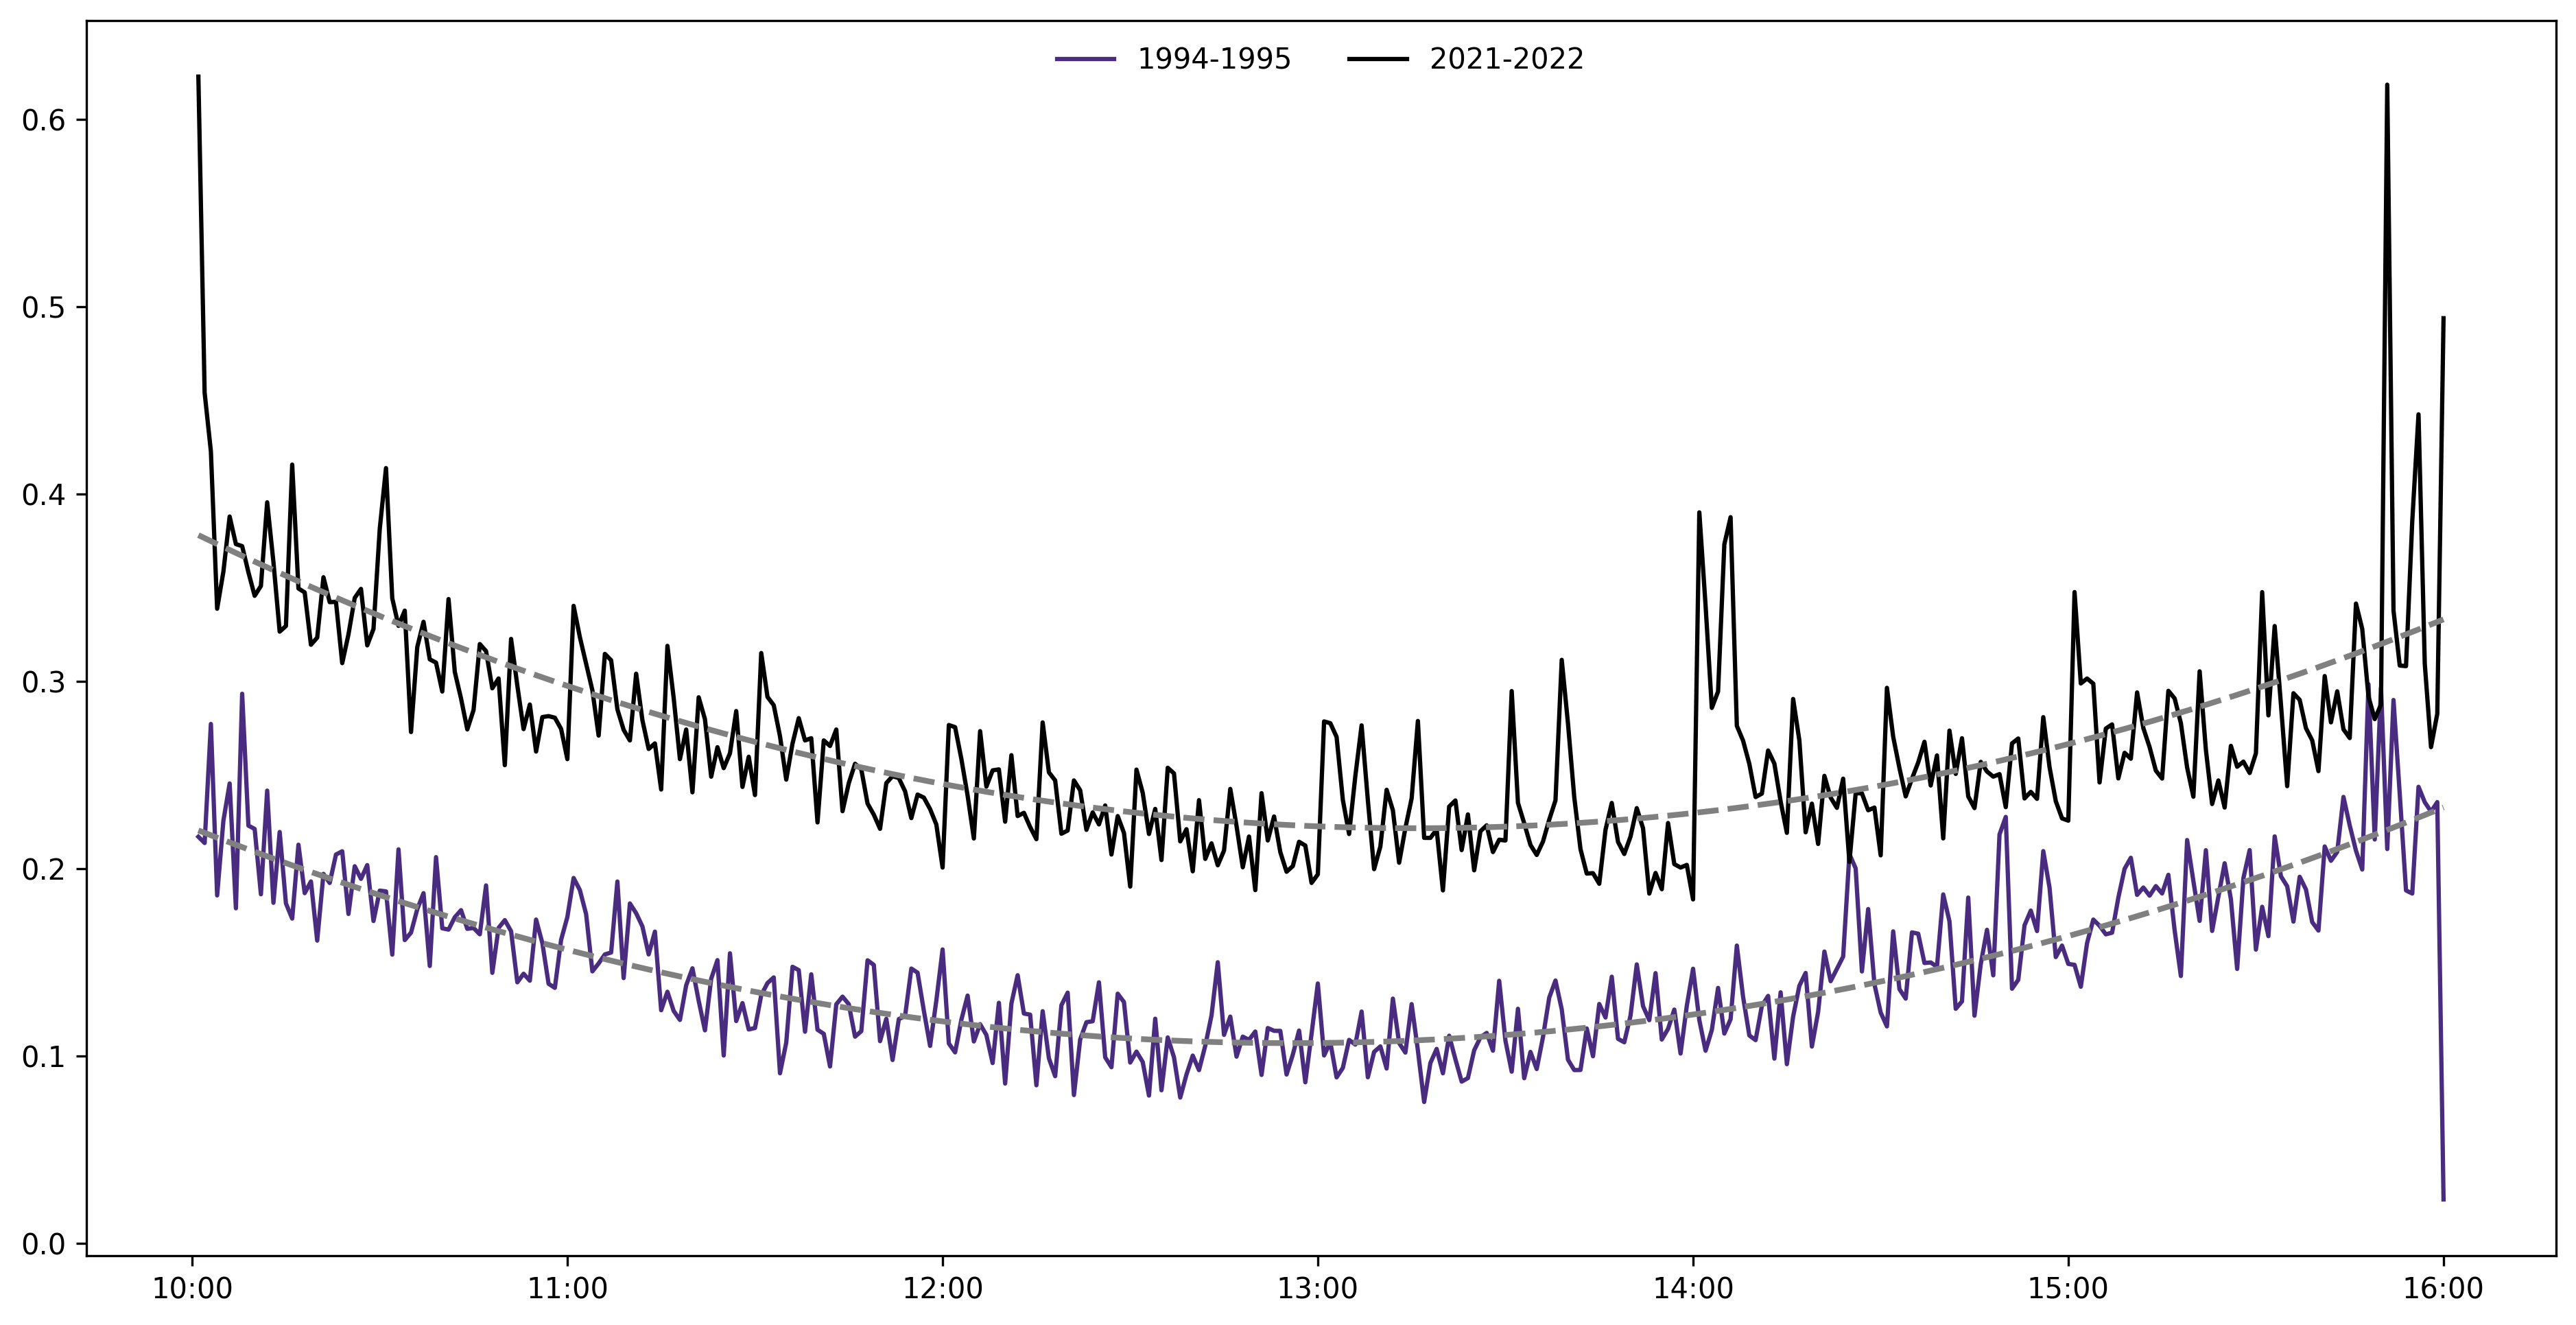
\includegraphics[width=0.8\textwidth]{images/intraday_vol_firstlast.png}
        \end{figure}
        
    \end{solution}
    \item Plot the time series of trading day RV measures for the full sample. Do this both for the regular RV measure (cumulative squared returns), but also for the square-root of the trading day RV, and the logarithm of the trading day RV. Compute the auto-correlogram for lags 1 through 20 of these series.
    
    \begin{solution}
        Figure~\ref{fig:realized_volatility} displays the three measures of volatility for the full sample as well as their 30 days moving average (MA). We can see that the volatility is very high in the 2000 and 2008 crisis and in the 2019 pandemic. The volatility clusters also seem very present in our sample as higher spikes are clustered around each other. 

        In terms of persistency, Figures~\ref{fig:realized_volatility_acf} and \ref{fig:realized_volatility_pacf} show the correlogram for the three measures of volatility. We can see that the volatility is highly persistent as the ACF and PACF decay very slowly for all of them. This is consistent with the stylized fact that volatility clusters. Moreover, the log and realized volatility (squared root) seem to have a higher persistency than the regular realized variance as displayed by their longer lasting autocorrelation.
        
        \begin{figure}[!htbp]
            \centering
            \caption{Trading Day Volatility Measures}
            \label{fig:realized_volatility}
            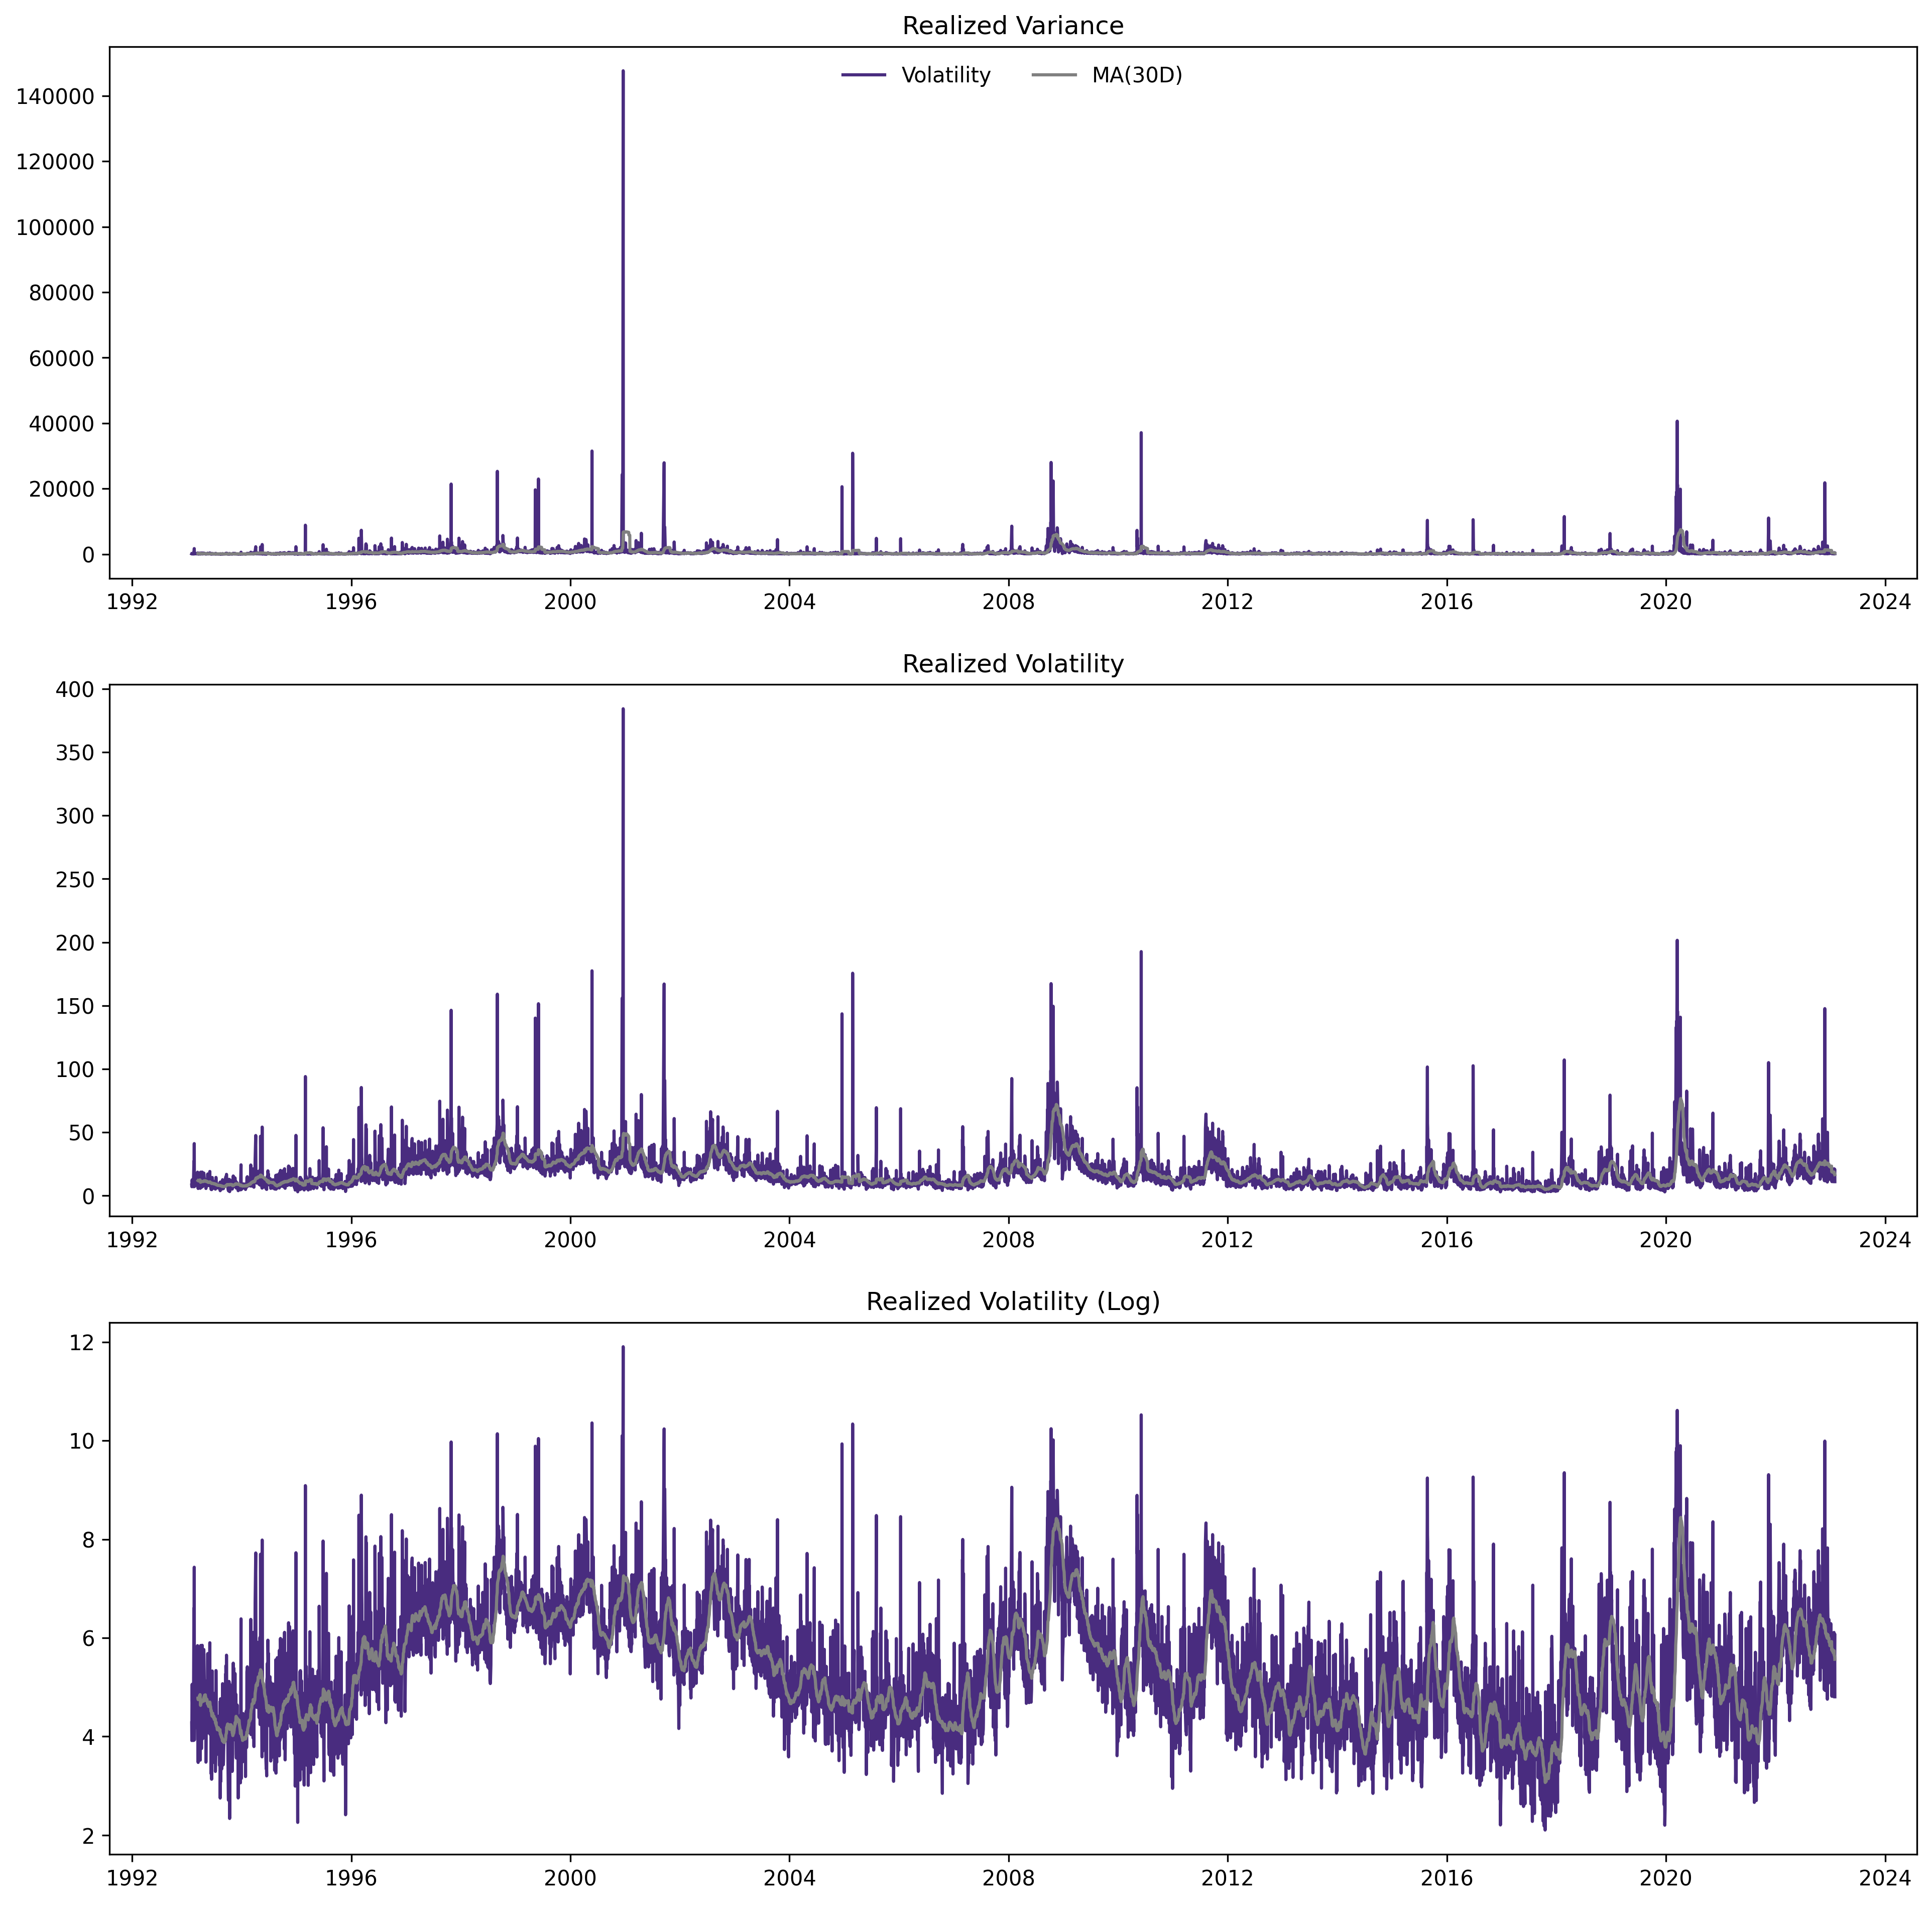
\includegraphics[width=0.8\textwidth]{images/realized_volatility.png}
        \end{figure}
        
        \begin{figure}[!htbp]
            \centering
            \caption{AutoCorrelation Function (ACF) of the Realized Volatility}
            \label{fig:realized_volatility_acf}
            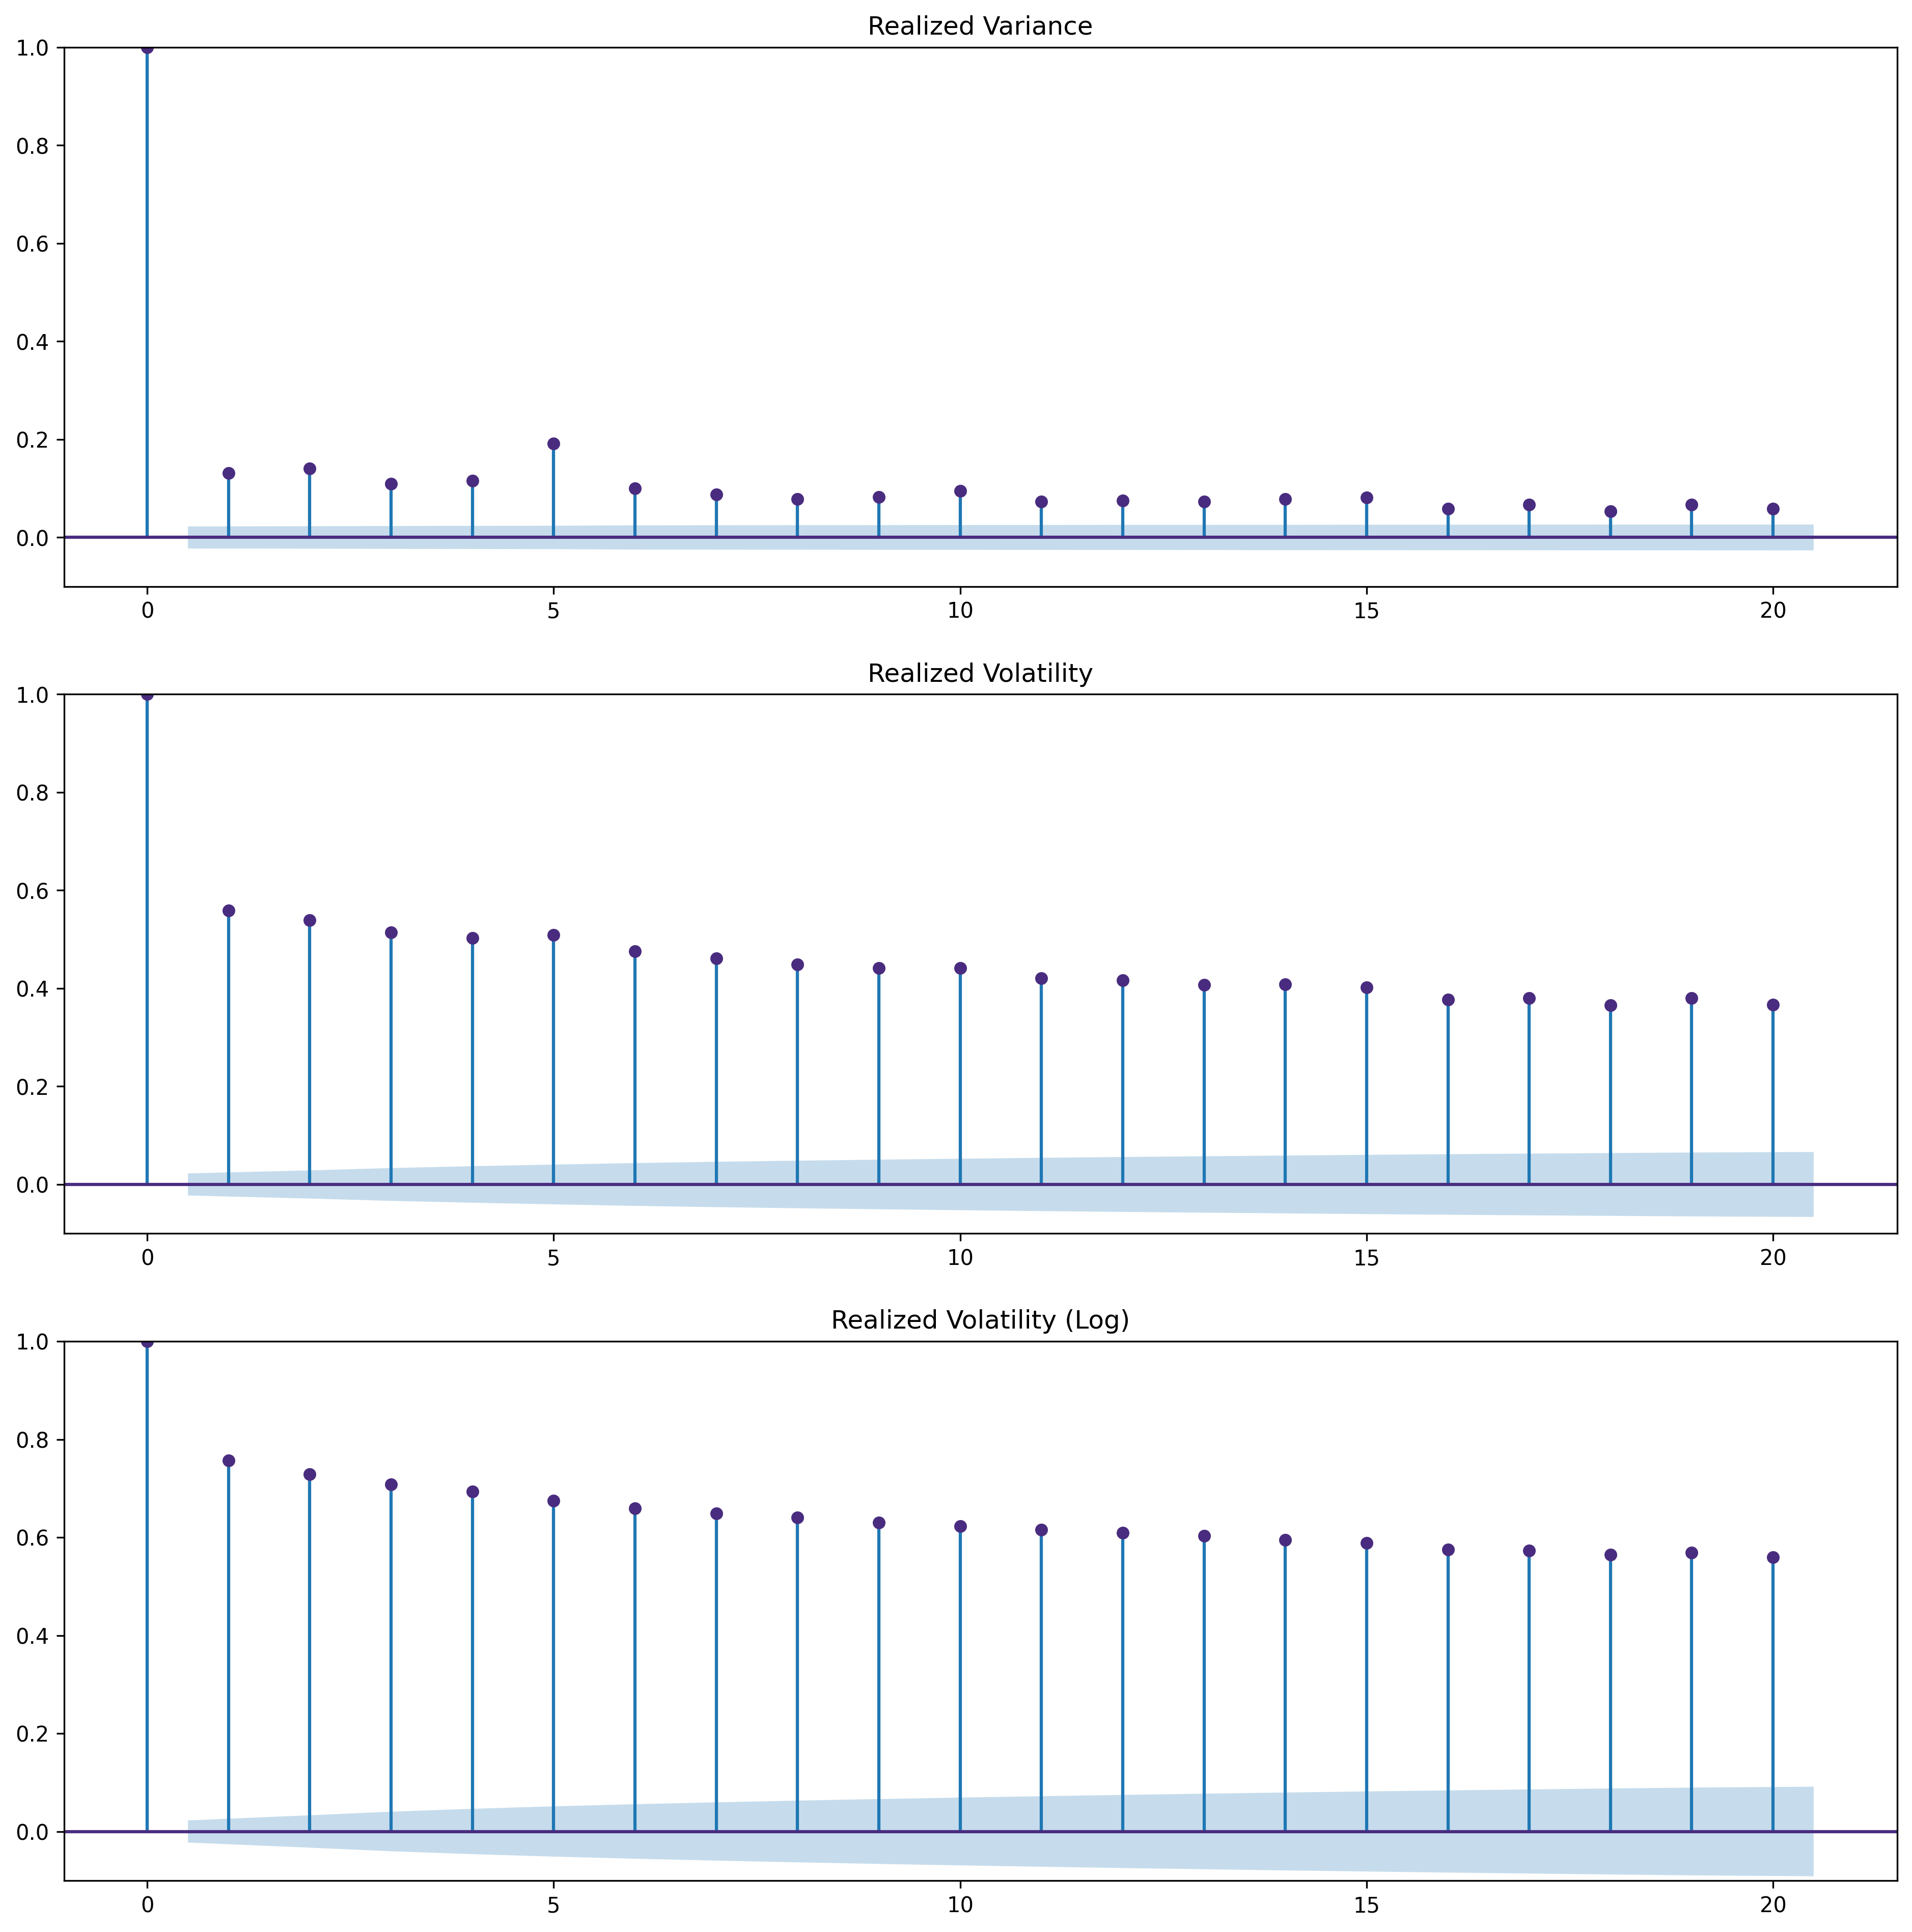
\includegraphics[width=0.8\textwidth]{images/realized_volatility_acf.png}
        \end{figure}
        
        \begin{figure}[!htbp]
            \centering
            \caption{Partial AutoCorrelation Function (PACF) of the Realized Volatility}
            \label{fig:realized_volatility_pacf}
            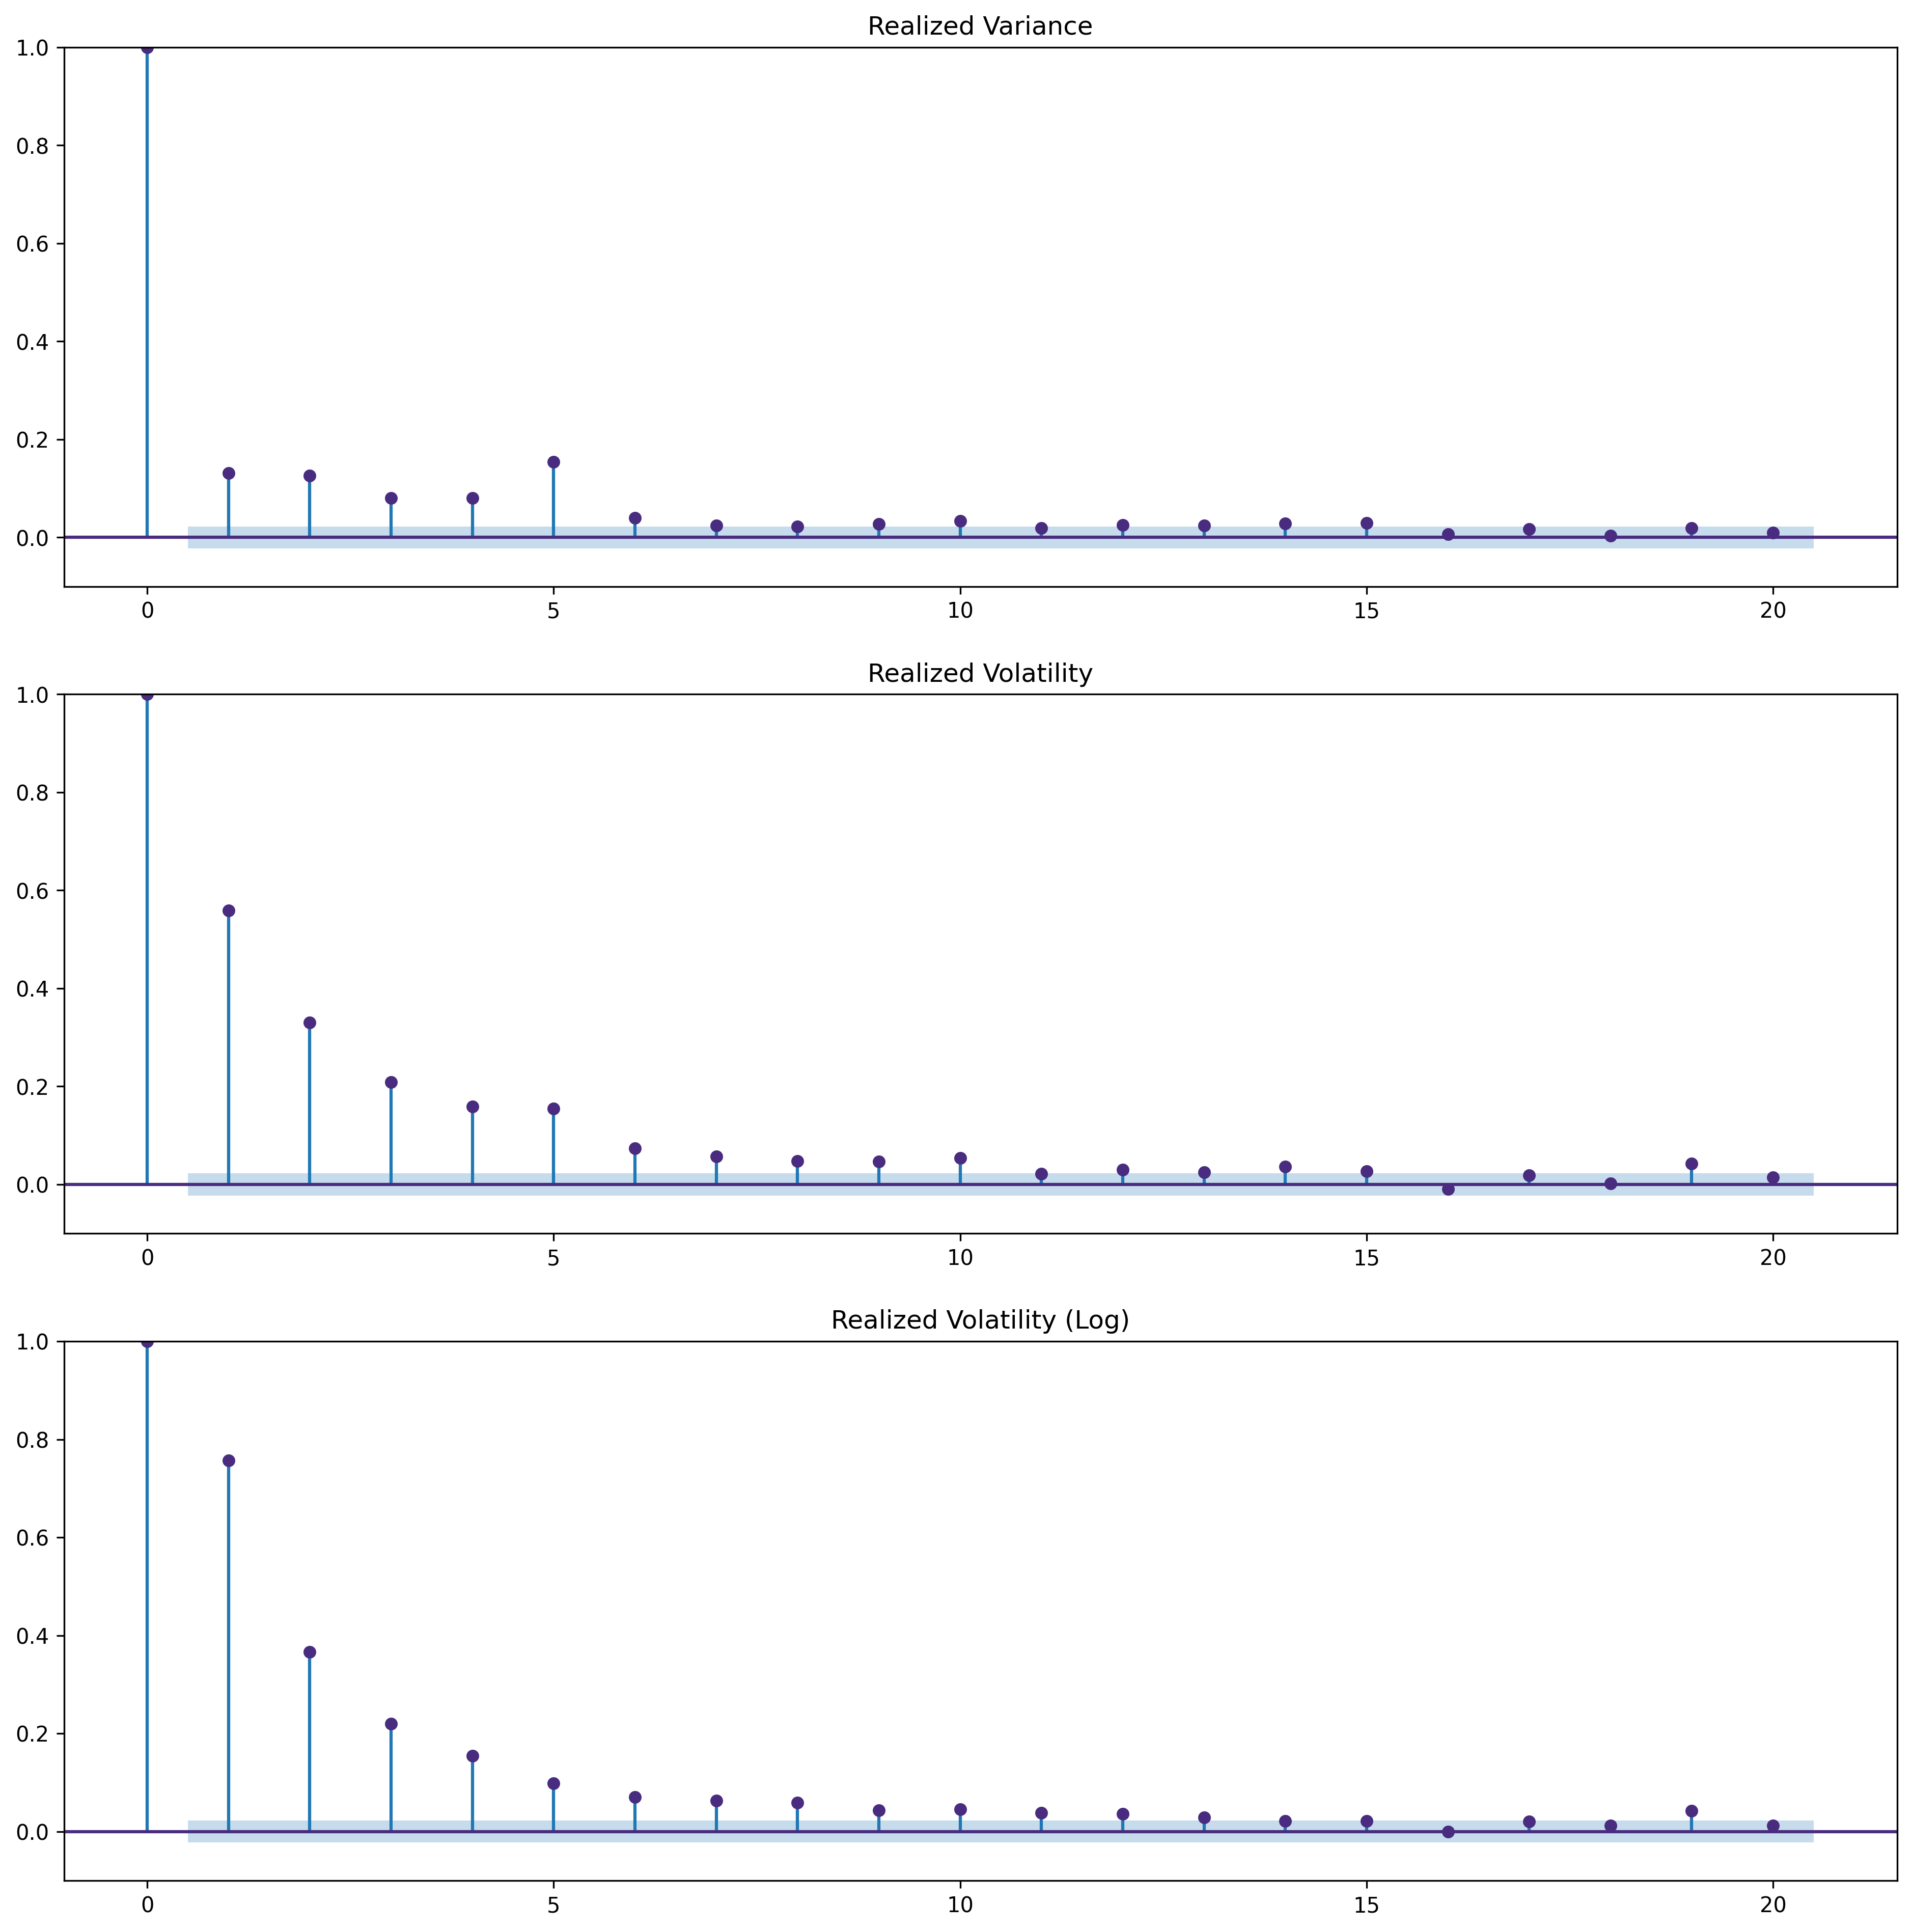
\includegraphics[width=0.8\textwidth]{images/realized_volatility_pacf.png}
        \end{figure}
        
    \end{solution}
\end{enumerate}
\end{document}